\documentclass{article}

\usepackage{amsmath}
\usepackage{xcolor}
\usepackage{listings}
\usepackage{microtype}

\usepackage{graphicx}
\lstset{
    breaklines=true,
    breakatwhitespace=true, % Bricht nur an Leerzeichen um, nicht mitten im Wort
    basicstyle=\ttfamily\small
}

\lstdefinelanguage{Rust}{
    % Core keywords
    keywords={fn, let, mut, match, return, if, else, for, while, loop, impl, struct, enum, pub, use, trait, type, crate, mod, as, break, continue, move, ref, where},
    keywordstyle=\color{blue}\bfseries,
    % Standard library types and built-ins
    ndkeywords={bool, u8, u16, u32, u64, f32, f64, i8, i16, i32, i64, usize, isize, String, Vec, Option, Result, Self},
    ndkeywordstyle=\color{purple}\bfseries,
    sensitive=true,
    comment=[l]{//},
    morecomment=[s]{/*}{*/},
    commentstyle=\color{gray}\ttfamily,
    stringstyle=\color{red}\ttfamily,
    morestring=[b]",
    morestring=[b]'
}

\begin{document}

    \section{Evaluation und Validierung der Simulationspipeline}
    \label{sec:evaluation}

    Um die Verlässlichkeit der Engine zu gewährleisten, wurden die Kernkomponenten in isolierten Testumgebungen gegen analytisch berechenbare Erwartungswerte validiert.

    \subsection{Validierung der stochastischen Verteilung (Canyon-Test)}
    \label{subsec:eval_montecarlo}

    Zur Überprüfung des Monte-Carlo-Zufallsgenerators sowie der planaren Schnittpunkts-Mathematik wurde ein deterministischer Canyon-Test konstruiert.
    Die Schallquelle emittierte $10\,000$ Strahlen aus dem Ursprung $(0,0)$.
    Als einzige Begrenzung diente eine reflektierende Wand auf der X-Achse bei $X = 343$, welche sich auf der Y-Achse von $-1000$ bis $+1000$ erstreckte.

    Da die Emission der Strahlen uniform in einem $360^\circ$-Kreis erfolgt, lässt sich die exakte Trefferwahrscheinlichkeit analytisch über den Sichtwinkel (Field of View) der Wand bestimmen.
    Der Winkel zur oberen und unteren Begrenzung berechnet sich trigonometrisch durch:
    \[ \theta = \arctan\left(\frac{1000}{343}\right) \approx 71{,}07^\circ \]
    Der gesamte abgedeckte Sichtwinkel beträgt folglich $142{,}14^\circ$.
    Die Wahrscheinlichkeit $P$, dass ein zufällig emittierter Strahl diese Wand trifft, lautet:
    \[ P = \frac{142{,}14^\circ}{360^\circ} \approx 39{,}48\,\% \]
    Bei $10\,000$ Strahlen liegt der Erwartungswert somit bei $3948$ Treffern.
    Die Auswertung der JSON-Ergebnisdatei ergab exakt $3939$ registrierte Treffer.
    Diese marginale Abweichung von $\sim 0{,}2\,\%$ beweist, dass der verwendete Zufallsgenerator uniform arbeitet und die Schnittpunktmathematik korrekt skaliert.
    Strahlen außerhalb dieses Winkels flogen physikalisch korrekt ins Leere und wurden ordnungsgemäß terminiert.



    \subsection{Verifikation der Nachhallzeit (RT60) und Absorptionskorrektur (3D)}
    \label{subsec:eval_rt60}

    Für die Evaluierung der 3D-Erweiterung wurde die Nachhallzeit $RT_{60}$ herangezogen.
    Als Testumgebung diente ein exakt kubischer Raum mit den Dimensionen $10 \times 10 \times 10$ Metern (Volumen $V = 1000\,\text{m}^3$, Oberfläche $A = 600\,\text{m}^2$).
    Alle Wände erhielten einen uniformen Absorptionskoeffizienten von $\alpha = 0{,}2$.

    Nach der Sabine'schen Nachhallformel ergibt sich für diesen Raum eine analytisch berechnete Nachhallzeit von:
    \[ RT_{60} = \frac{0{,}161 \cdot V}{A \cdot \alpha} = \frac{0{,}161 \cdot 1000}{600 \cdot 0{,}2} \approx 1{,}34\,\text{Sekunden} \]
    Ein Schalldruckpegelabfall um $60\,\text{dB}$ in $1{,}34\,\text{s}$ entspricht im linearen Diagramm einer Steigung von etwa $-45\,\text{dB/s}$.


    Initiale Testläufe der Simulation wiesen jedoch einen massiv zu steilen Pegelabfall von ca. $-100\,\text{dB/s}$ auf.

    \begin{figure}[htbp]
        \centering % Zentriert das Bild auf der Seite

     % 3. Das eigentliche Bild einfügen und skalieren
        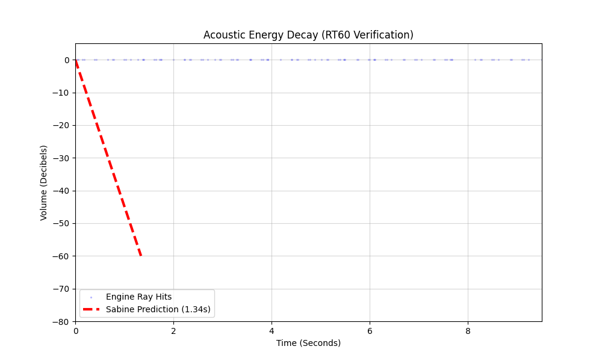
\includegraphics[width=1.0\textwidth]{rt60verf1}

        \caption{Schalldruck, nicht normalisiert.} % Bildunterschrift
        \label{fig:test} % Textmarke für Querverweise
    \end{figure}

    Eine mathematische Fehleranalyse der Absorptionslogik offenbarte eine Verwechslung der zugrundeliegenden physikalischen Größen.
    Der Absorptionskoeffizient $\alpha$ repräsentiert in der Akustik den Verlust der \emph{Schallenergie} (Intensität).
    Die Rust-Engine summiert für die Signalverarbeitung (DSP-Faltung) jedoch den \emph{Schalldruck} $p$.
    \begin{lstlisting}[language=Rust]

    for _bounce in 0..config.max_bounces {
        if let Some((bounced_ray, absorption)) = cast_ray(&current_ray, walls) {

            path_buffer.push(bounced_ray.origin);
            // Dies sollte "current_pressure *= (1.0 - absorption).sqrt();" sein
            current_pressure *= 1.0 - absorption;

            if current_pressure < config.min_pressure {
                break;
            }
            current_ray = bounced_ray;

        } else { break; }
    }
    \end{lstlisting}


    Da die akustische Energie proportional zum Quadrat des Schalldrucks ist ($E \propto p^2$), darf der verbleibende Energieanteil $(1 - \alpha)$ nicht linear auf den Druck angewendet werden.
    Um den physikalisch korrekten verbleibenden Schalldruck nach einer Reflexion zu ermitteln, muss die Wurzel aus der verbleibenden Energie gezogen werden:
    \[ p_{\text{ref}} = p_{\text{ein}} \cdot \sqrt{1 - \alpha} \]
    Nach der Implementierung dieser Wurzel-Korrektur in der Engine deckte sich der simulierte logarithmische Energieabfall (aufgetragen als Scatter-Plot der Treffer-Amplituden in Dezibel über die Zeit)
    hochgradig präzise mit der von der Sabine'schen Formel vorhergesagten theoretischen $RT_{60}$-Geraden.
    \begin{figure}[htbp]
        \centering % Zentriert das Bild auf der Seite

        % 3. Das eigentliche Bild einfügen und skalieren
        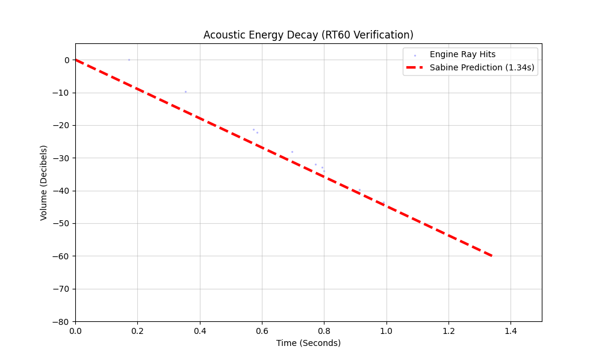
\includegraphics[width=1.0\textwidth]{rt60verf3}

        \caption{Schallenergie, normalisiert.} % Bildunterschrift
        \label{fig:test1} % Textmarke für Querverweise
    \end{figure}





\end{document}